% !TEX root = ..\thesis.tex
\chapter{绪论}\label{chap:introduction}

\section{研究背景及意义}

近来,随着软件过程管理、互联网模式的不断发展与更新,软件应用的数量以及规模的不断扩大,软件应用的迭代也不断加快,如何迅速及时地发现高质量的软件需求,并对其进行准确的识别和抽取成为开源社区以及业界需要解决的问题 \cite{Saur2006Review}。


IEEE软件工程中定义需求为:用户解决问题或达到目标所需的条件和能力;系统或系统部件为满足合同、标准、规范或其它正式规定文档所需具有的条件和能力;以上条件和能力的文档说明 \cite{Board2002IEEE}。软件需求可分为业务需求、用户需求、功能性需求、非功能性需求、设计约束、系统约束等。


需求发现和抽取是指收集准备建立的系统和正在使用的系统的信息,并从这些信息当中提取用户和系统需求 \cite{Vlas2011A}。需求的获取应注意三个方面:应获取的信息,使用的信息来源,采用的获取技术。为了收集到全面完整的信息,需求获取可以通过对现有系统分析、与潜在用户和购买者交流、讨论等方式来导出软件系统的需求。需求发现阶段的信息源包括已有文件、系统信息持有者以及类似系统的相关内容。需求的获取有多种渠道,比如可以通过市场调研的方式,从市场走向分析以及从产品走向分析,确定用户的相关需求和边际需求;也可以开发一个或者多个系统模型或原型来帮助用户更好的表达系统的需求 \cite{唐中君基于},这样有利于系统分析员了解所要描述的系统的功能;需求人员还可以把自己作为系统的最终用户,审视该系统并提出问题,但这需要需求人员具有比用户更多的应用领域和过程管理方面的知识,并具有良好的想象能力;为了确定系统应该具有的功能,需求人员通过提出问题和用户回答,直接询问用户想要的是什么样的系统;观察是另一种需求获取的方法,通过观察用户执行其现行的任务和过程,或者通过观察他们如何操作与所期望的新系统相关的现有系统,了解系统运行的环境,特别是了解要建立的新系统和现存系统、过程以及工作方法之间的必须进行的交互;另一种方式是通过小组会的方式,可以举行客户和开发人员的联席会议,与客户组织的一些代表共同开发需求;另外还可以通过提炼的方式获取需求 \cite{孙挺2002基于},提炼方法是针对已经有了部分需求文档的情况,复审技术文档,例如有关需求的陈述功能和性能目标的陈述,系统规约接口标准,硬件设计文档,以及ConOps文档,并提出相关信息。在特定的环境中,每项技术都有其自己的优点和不足,在实施上述任何一项技术时,都可以辅以其他方法,比如原型构造,在举行小组会时可以使用原型,方便人员之间的交流。依据需求工程人员的技能和产品、合同的实际情况,往往需要组合使用这些技术来开发初始需求。执行需求发现这项活动的人,其技能水平对这项活动的成功也具有巨大的影响。

% 在当今许多开源项目和工业软件中,开发者大量使用交流平台, 比如邮件,问题追踪,聊天等 \cite{panichella2014developers}表达他们的去定义软件的特征的需求\cite{fitzgerald2006transformation}。在这些数据中包含的信息已经被研究者用来构建推荐系统,比如缺陷追踪系统、自动为项目经理提供建议和为一个软件制品自动生成描述等。



如今,软件应用服务的开发者和用户会根据他们的感知体验质量,以简短的评论和排名的形式提供反馈,甚至参与由社交媒体或基于Web的专用交流支持的在线讨论平台,例如在线聊天、App Store、用户论坛、邮件列表、Wiki,新闻组和博客。 这种在线用户反馈的数量迅速增加,成为软件数据的重要组成部分,并且可以通过软件分析支持软件工程中的决策,从而推动软件工程研究的发展\cite{Morales2019Speech}。 
伴随着这一趋势,在需求工程(RE)中,提出了基于群体的需求工程(CrowdRE)\cite{groen2017crowd}范式,该范式定义了收集,分析和管理群体表达的需求所需的概念,方法和技术集。


最近的研究报告表明,在包括邮件、issue tracker等各种交流平台中,在线聊天的使用越来越流行,并且在软件开发中起着越来越重要的作用,在某些情况下已经取代了电子邮件\cite{lin2016developers}。开发人员正在转向公共工作聊天平台,例如Slack、IRC、HipChat、Gitter和Freenode,以在上面分享观点和有趣的见解、讨论如何解决缺陷以及将来要实现的功能\cite{chatterjee2019exploratory}。在线聊天中开发人员通常会在对话中向其他开发者提出其所希望实现的功能,如图\ref{fig:motivation}所示,以AngularJS项目中的聊天消息为例,开发人员P和F在在线聊天中发布了他们的问题。最初,他们的意图是寻求其他开发人员的帮助,以寻求可行的解决方案。但是在与其他开发人员聊天之后,他们意识到现有系统无法实现他们的要求。然后,他们的意图从寻求解决方案转变为提出需求。P请求“交互性复选框的ng-true-value / ng-false-value之类的东西”,F表示“angular cli可以将我的所有服务放入服务文件夹”。
\begin{figure}[htbp]
    \centering
    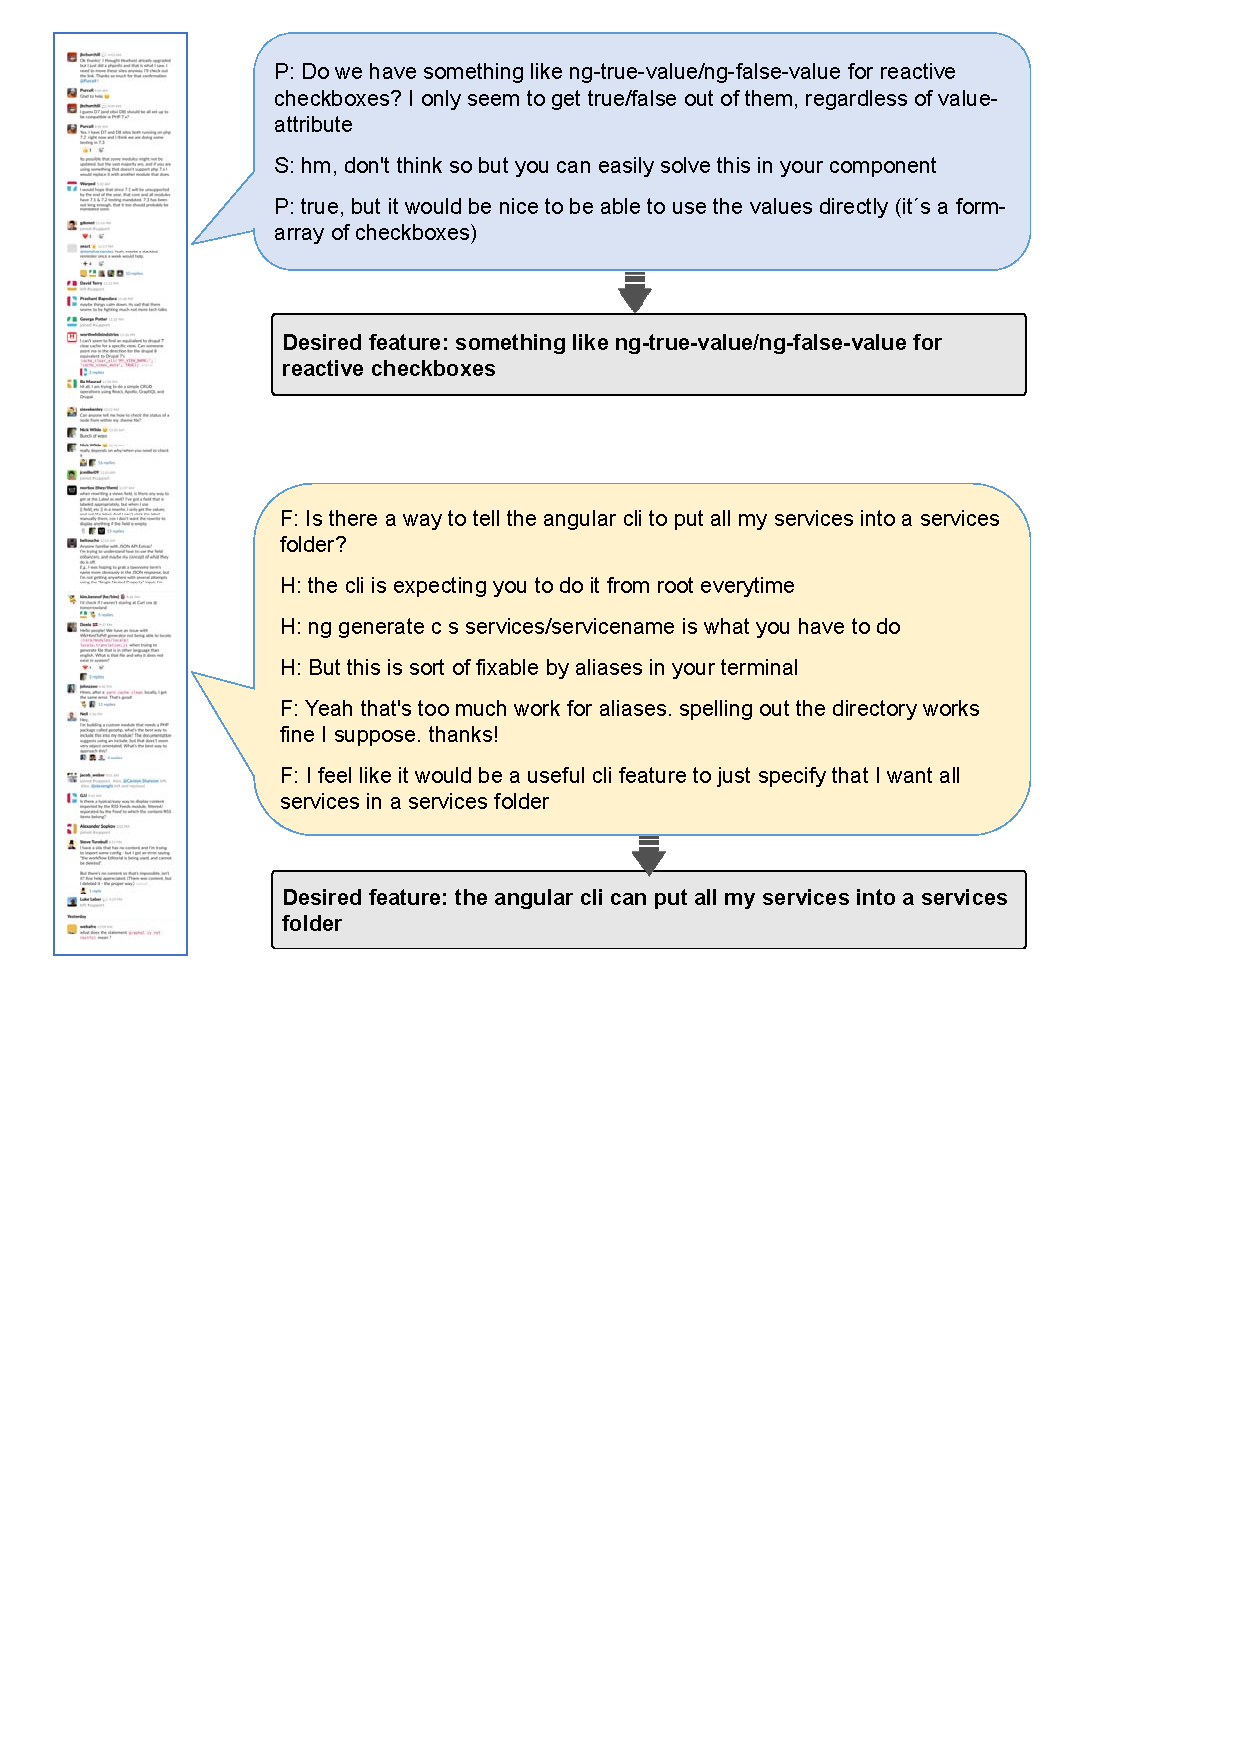
\includegraphics[width=0.70\textwidth]{Img/motivation.pdf}
    \bicaption{AngularJS项目的一个聊天信息例子,需求淹没在大量聊天历史中}{Example chat message from AngularJS project, where requests to desired features are buried in the massive chat history.}
    \label{fig:motivation}
\end{figure}
为统一表示,下文中将使用“\textbf{需求对话}”表示如图\ref{fig:motivation}所示的这种开发者之间在讨论新功能、完善功能的聊天对话。

虽然理解开发人员在文本对话中讨论的需求可以为开源项目提供启发和见解,但是手工对自然语言需求进行分析是十分耗时的,在大型项目中甚至会产生错误\cite{vlas2012two},并且由于在线聊天的开放性和实时性,这些需求对话很快就会被新收到的消息淹没。通常情况下,如果在线聊天中讨论的需求未被开发人员记录在文档中,则其很可能会被淹没或忽略。因此,自动对聊天记录中的隐藏需求进行分析和挖掘会带来巨大的好处并减少开发人员的时间成本。
实际上,发布团队会监视各种沟通渠道,以获取与下一个发布版本可能相关的信息。如果发布团队可以从聊天消息中确认那些隐藏的需求,则为了最大化利益相关者的满意度,他们的下一个发布计划可能会考虑实现更多的需求。

通过应用从大量的聊天消息中检索有价值信息的自动化挖掘技术,开发人员可以从大量用户那里收集全面的需求,这有助于发布团队对需求的确定和发布版本计划,进而促进软件开发的成功。尽管聊天消息数据源可能很庞大,并且随着时间的推移加入了了越来越丰富的新需求,但是由于以下困难,要从大量的聊天消息中挖掘隐藏需求还是非常具有挑战性的。
\begin{enumerate}
    \item \textbf{对话层次分析:}不同于常规的句子级别的文本挖掘任务,当分析来自聊天消息的对话时,对于理解一个句子,需要考虑对话范围内的上下文信息。因此,关于句子级别需求发现的现有研究不能直接用于此任务。例如,“我们需要添加垂直导航栏选项”被句子级别技术分类为需求意图。但是,当在在线聊天中发出此对话时,后续对话指出现有功能可以以替代的方式满足该请求。此外,句子级别的分类结果是不准确的,因为其在聊天消息中将大量离题句子识别为需求意图,例如,“我真的需要恢复我的编程技能”,“我想喝点咖啡和饼干”,这些句子在表达其愿望,但并非为需求。
    \item \textbf{极其昂贵的标注:}聊天消息通常规模很大。在大量聊天消息中查找需求对话,就像在大海捞针一样。由于庞大的语料库和少量的正样本数据,只有少数聊天消息为需求类型,因此标注聊天消息中的需求对话所需成本极其昂贵。如何最大程度地利用少量标注数据来对未标注聊天消息进行准确分类成为一个关键问题。
    \item \textbf{耦合和噪声数据:}聊天消息通常是大规模的,并且是包含涉及广泛主题的非正式对话。两个或多个开发人员彼此同步地进行交互,其中他们的对话在聊天记录中很大程度上被耦合。此外,在聊天消息中存在噪声文本,例如重复消息和离题消息,这些消息不会提供任何有价值的信息。因此,耦合和噪声数据给分析和理解对话带来了巨大的困难。
\end{enumerate}

\section{研究内容和创新点}

因为用户和开发者之间、公司开发者团队内部之间等通常最先在开放式聊天平台显式或潜在地提出需求,里面会存在着大量的原始需求。并且聊天数据量一般较大,蕴含时间、用户角色等对需求十分重要的信息。因此,聊天数据作为需求的一个典型来源,一般团队会要求开发者在会话期间记录需求。本工作可以从聊天数据中挖掘出隐藏的大量的用户需求对话,对通过传统需求发现的方式起到了启发、补充等作用。观察解耦后的会话可看出,对话中需求的表达形式因角色、上下文的不同而不同,有些显式地表达出清晰的需求,有些较为隐式地或者在交谈过程中逐步确定需求,因此,根据传统的基于规则或者统计机器学习方式的需求识别方法很难以及不能完整地识别并抽取需求,对此,本工作使用深度学习基于对话形式进行需求识别和抽取。


本文将主要从开放式聊天平台的数据出发,因聊天数据的规模较大、需求表述不规范、不明确、需求稀疏等问题,本文结合需求工程以及自然语言处理、机器学习等技术抽取出需求对话,并对其进行推荐,以达到快速及时发现需求的目的,其可以减少开发人员在聊天过程中对需求的记录,避免丢失重要的关于需求的信息,并对传统需求发现方式起到启发,补充的目的。

本工作是首先在对话级别上进行分析的方法,其旨在自动检测聊天消息中发布的隐藏的需求。本文提出了一种名为{\tool}的新方法,该方法可以通过深层孪生网络从聊天消息中识别隐藏的需求对话。为了更好地理解对话级别的上下文信息,本文首先基于双向LSTM(BiLSTM)结构构建了一个上下文敏感对话模型{\dm},该模型可以深入学习正向和反向对话的上下文信息。受到利用少量标注样本来建立预测模型技术的启发,本文把传统文本分类任务转换为确定两个对话是否属于同类的任务。因此,{\tool}将上下文敏感对话模型与孪生网络相结合,以学习一对对话之间的相似性,而不是单一对话类别。需求对话的预测结果可以基于相似性预测结果,及其配对对话的类别来推断。为了评估本文提出的方法,标注团队标注了三个流行的开源项目中的1,035个对话。实验结果表明,本文的方法明显优于两个句子级别需求分类模型和四个传统文本分类方法,其平均精度,召回率和F1值分别为88.52%,88.50%和88.51%。结果证实,{\tool}可以有效地检测聊天消息中的隐藏需求,从而可以自动方式从大量用户收集全面的需求。

本文主要贡献主要有以下几方面:
\begin{enumerate}
    \item  本文是首先提出从大量聊天消息中识别隐藏需求的,这些需求可以帮助发布团队进行全面的需求收集。
    \item 本文引入了一种解决方案,其可以通过结合孪生网络来基于有限的标注数据有效地识别需求对话,从而大大减轻了对数据进行标注的负担。
    \item 本文在三个活跃的开源项目中评估了{\tool},并进行了实验比较,结果表明{\tool}优于现有的需求挖掘方法和四个文本分类方法。
    \item 发布了可公开访问的数据集和源代码\footnote{https://github.com/FRMiner/FRMiner},以促进本文的研究及其在进一步研究下的重用。
\end{enumerate}



\section{论文组织结构}
本文内容共分为六章,章节之间逻辑关系如图\ref{fig:chapters}所示。
\begin{figure}[htb]
    \centering
    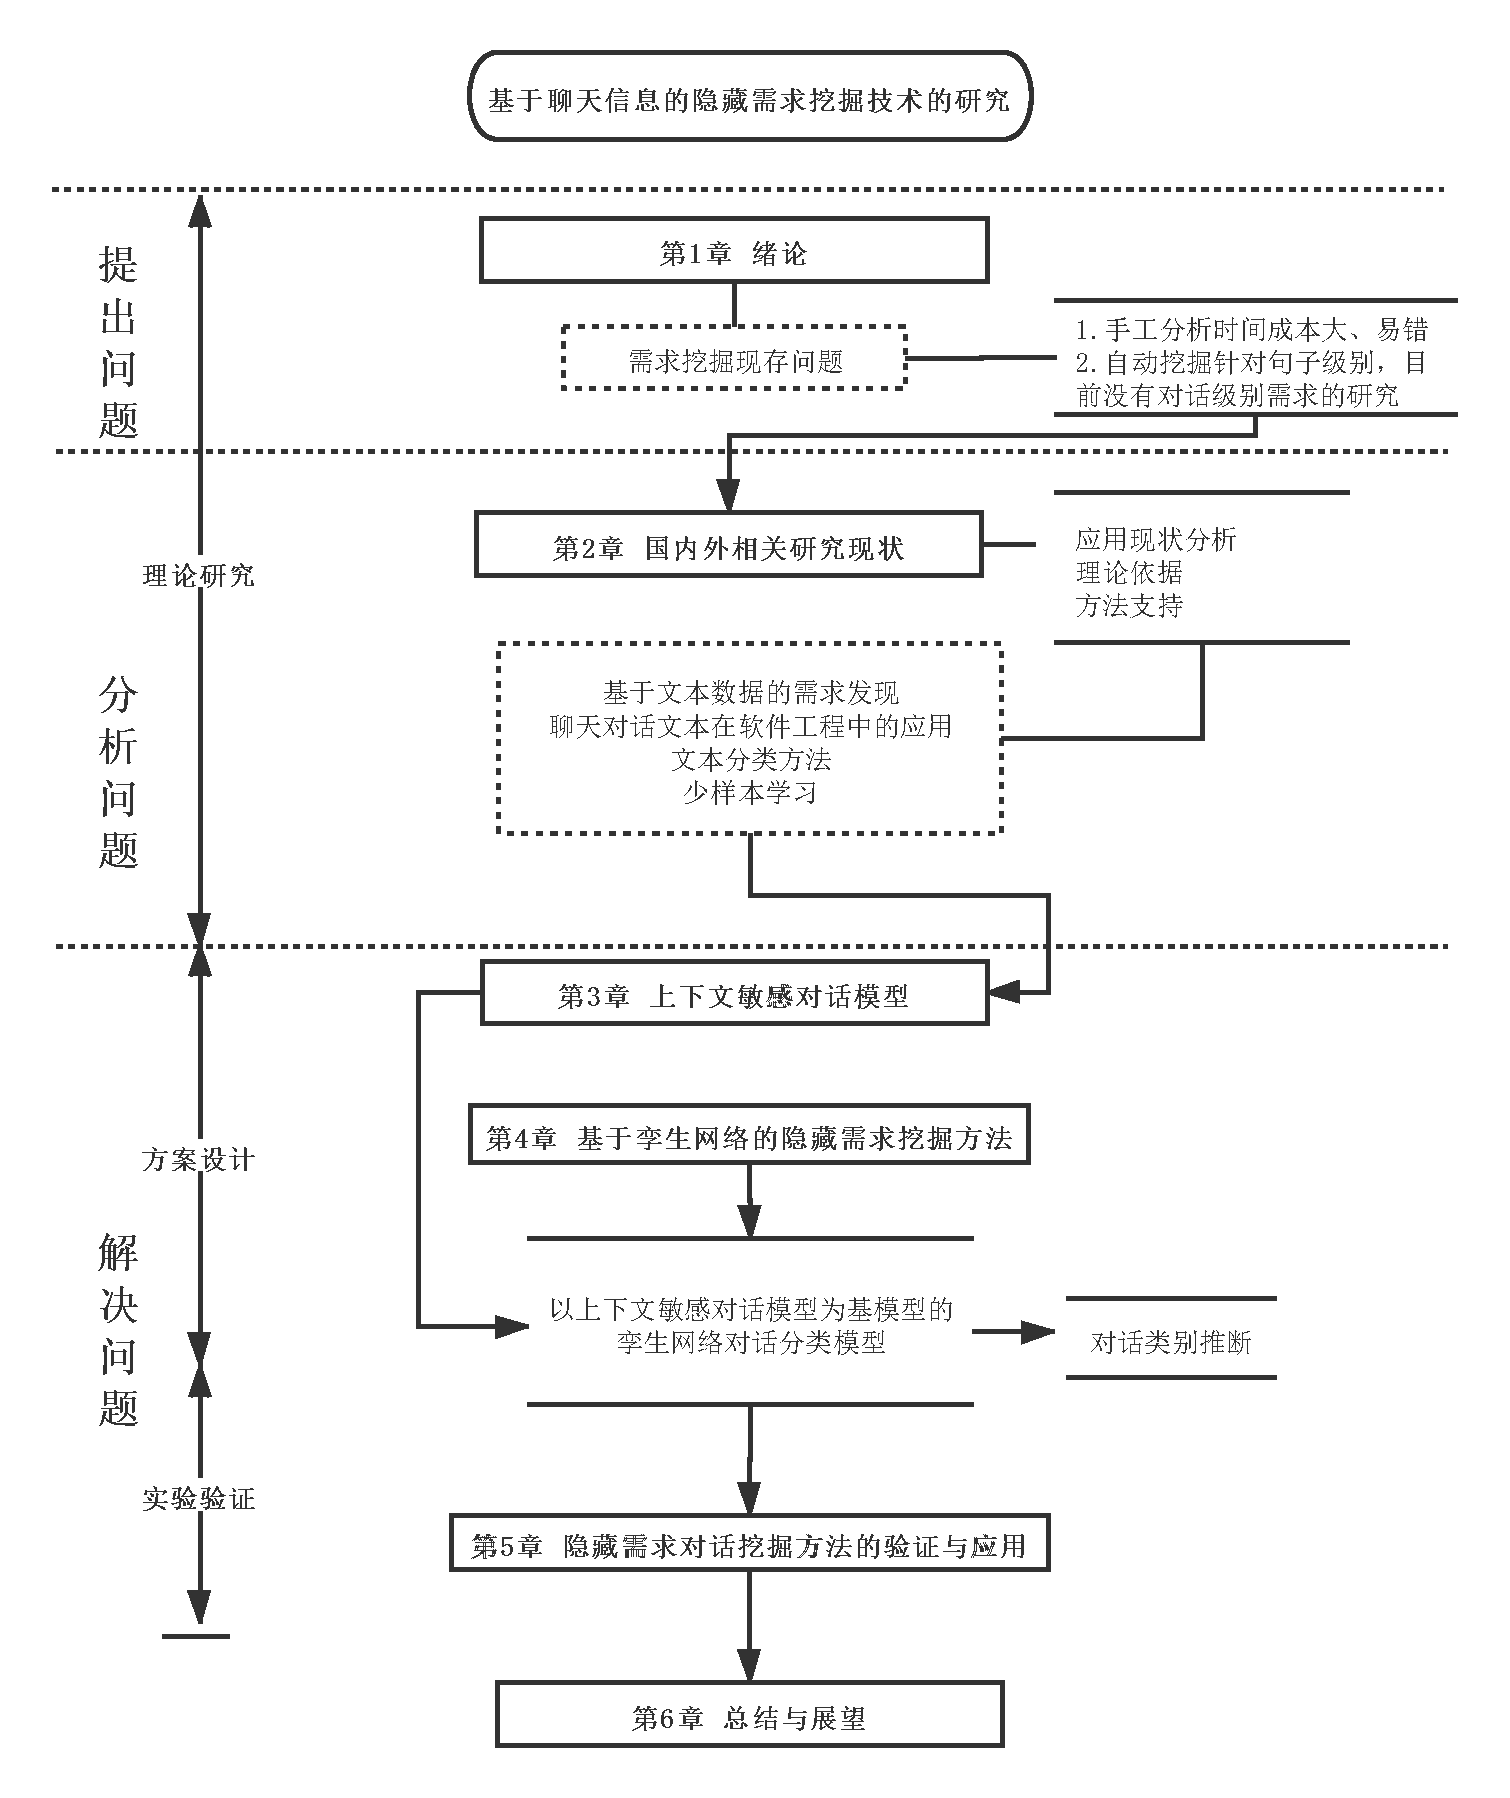
\includegraphics[width=0.8\textwidth]{Img/chapters.pdf}
    \bicaption{本文章节结构}{The relationships among chapters in this paper}
    \label{fig:chapters}
\end{figure}

各章节的具体内容概述如下: 

第 1 章 绪论 

本章目的在于阐述从大规模聊天记录中进行需求自动识别和抽取的研究背景及研究意义,并对本文的主要研究内容以及创新点进行归纳。通过论述需求对话自动抽取的研究背景
及意义论证需求对话自动化识别的可行性以及必要性。并针对从大规模聊天记录中进行需求对话识别过程中存在的三大问题,即对话层次分析、标注成本大和噪声数据多提出本文的基于孪生网络和分层上下文敏感对话模型{\dm}的{\tool},并介绍了本文的贡献点。以及通过介绍本文的组织架构对全文内容进行总结。 

第 2 章 国内外相关研究现状

本章目的在于介绍近年来围绕着需求发现的工作,主要包括基于手工设计规则和基于统计机器学习的方法。接下来介绍聊天对话文本在软件工程中的应用。接下来介绍了自然语言处理中常见的分类方法,并对于对话标注困难、标注数据量少的问题介绍了少样本学习。

第 3 章 上下文敏感对话模型

本章目的在于介绍对话解耦这一对话分析中必不可少的关键步骤,并针对本文中使用的对话解耦方法展开介绍;接下来,针对对话模型,本章从不同层次展示了本文设计的上下文敏感对话模型{\dm},该模型可以将解耦之后的对话进行向量化表示,并应用到本文的隐藏需求对话识别的任务中。


第 4 章 基于孪生网络的隐藏需求挖掘方法

本章目的在于介绍本文提出的{\tool}模型结构和类别推断。首先介绍了{\tool}的模型结构,如图\ref{fig:34relation}所示,其以第3章中介绍的上下文敏感对话模型{\dm}为基模型构建孪生网络。
然后为孪生网络构建针对Pair-Instance的分类器,并且大大增强了数据量。接下来介绍了针对Pair-Instance进行目标对话的类别推断。最后介绍了模型实现细节、参数微调优化。

% 第 4 章 需求对话识别模型数据集构建和模型实现

% 本章目的在于介绍从数据集爬取、文本预处理、对话解耦、数据标注的数据集构建过程。然后,分别介绍分层上下文敏感对话模型和孪生网络的工程实现。接下来,介绍了模型训练过程和参数微调。最后,本文说明了{\tool}在工业场景部署的步骤。

第 5 章 隐藏需求对话挖掘模型验证与应用

本章目的在于介绍从数据集爬取、文本预处理、对话解耦、数据标注的数据集构建过程。接下来介绍三个验证实验,即FRMiner的需求识别的有效性实验、孪生网络在FRMiner中的有效性实验、FRMiner的项目间泛化能力实验的实验设置,并针对实验结果进行分析,试验结果表明,本文方法在精确度、召回率、F1值上超越了包括两个先进的句子级别需求发现模型以及四个文本分类方法;并且对于孪生网络带来的数据增强,模型整体效果随着数据集增强而提高;另外也证明了{\tool}在不同项目间对需求对话模式的泛化能力。三个实验整体上论证了本文方法的有效性。最后,介绍了本研究中实现的{\tool}工具的离线、在线训练使用。

第 6 章 总结与展望

本章目的在于对全文内容进行总结,指出本文研究工作中可以进一步改进的地方,并介绍下一步工作进展计划。 


\section{本章小结}

本章通过论述本文的研究背景及意义证实了基于大规模聊天记录进行需求对话识别和抽取的可行性以及必要性。并针对目前需求识别过程中存在的问题提出本文的研究内容以及创新点。最后,通过介绍本文的组织架构对全文内容进行总结。 